\chapter{五维函数求极值}
\section{题目描述}

求解下面五维函数的最小值:
\begin{align}
f \left( x _ { 1 } , x _ { 2 } , x _ { 3 } , x _ { 4 } , x _ { 5 } \right) = \left( x _ { 1 } - 0.718 \right) ^ { 2 } + \left( \frac { x _ { 2 } + 0.718 } { 2 } \right) ^ { 2 } + \left( x _ { 3 } - 0.2 \right) ^ { 2 } + \left( \frac { x _ { 4 } + 2 } { 0.1 } \right) ^ { 2 } + x _ { 5 } ^ { 2 } + \left( x _ { 2 } - x _ { 3 } - 1.5 \right) ^ { 2 }
\end{align}

其中每个参数的范围是:
\begin{align}
x _ { 1 } \in [ - 1,1 ] , x _ { 2 } \in [ - 1,1 ] , x _ { 3 } \in [ - 5 , - 1 ] , x _ { 4 } \in [ 0,2 ] , x _ { 5 } \in [ - 2,2 ]
\end{align}

\section{题目分析}

这是一个典型的函数求极值的问题,我已开始写了一个最陡下降法来计算该五维函数的最小值,但是发现求出来的极值并不在题目给定的参数范围之内,所以只好重新找方法. 注意到我们其实可以把每个参数的范围限定看做是线性约束,也就是一阶不等式来处理:
\begin{align}
&x_1\geq -1, \qquad x_1\leq 1\\
&x_2\geq -1, \qquad x_2\leq 1\\
&x_3\geq -5, \qquad x_3\leq -1\\
&x_4\geq 0, \qquad x_4\leq 2\\
&x_5\geq -2, \qquad x_5\leq 2
\end{align}

也就是原最优化问题加上了10个线性约束. 常用于求解约束最优化问题的是 Frank-Wolfe 算法.

\subsection{Frank-Wolfe 算法}

Frank-Wolfe 算法常用于解决约束最优化问题.假设区域$D$是参数空间中取值的可行域,函数$f\colon {\mathcal  {D}}\to {\mathbb  {R}} $是$D$上的可微凸函数.Frank-Wolfe 可以解决以下最优化问题:

\begin{equation}
\min  {\displaystyle f(\mathbf {x} )} \qquad  \mathbf{x} \in \mathcal{D}.
\end{equation}

我们可以用泰勒展开对目标函数进行近似,将它线性化.将$f(x)$在$x_0$处展开,有:

\begin{align}
&\min f ( x ) \approx f \left( x _ { 0 } \right) + \nabla f \left( x _ { 0 } \right) ^ { T } \left( x - x _ { 0 } \right)\\
&\mathbf{x} \in \mathcal{D}.
\end{align}

去掉常量后,问题可以写为:
\begin{align}
&\min f ( x ) \approx \nabla f \left( x _ { 0 } \right) ^ { T } x\\
&\mathbf{x} \in \mathcal{D}.
\end{align}

设此问题的最优解为$y_i$,则直观上$d_i=y_i−x_i$ 应当为原问题的可行下降方向,沿着此方向做一维搜索则可进行一次迭代.为了防止一维搜索的结果超出可行域,我们限制步长$0 \leq \lambda \leq 1$.注意到线性规划的可行域为凸集,由于$x_i$和$y_i$均为可行点,它们确定的连线均在可行域中.限制步长$0 \leq \lambda \leq 1$保证了一维搜索的结果在可行域中.

具体算法步骤如下:
\begin{enumerate}

\item 选择初值。初始点$\mathbf{x_0} \in \mathcal{D}$,给定允许误差$\epsilon>0$,令$i=0$.

\item 求解近似线性规划:
\begin{array} { c l } { \min } 
& { \nabla f \left( x _ { i } \right) ^ { T } x } \\ 
&\mathbf{x} \in \mathcal{D}
\end{array}

得最优解$y_i$

\item 构造可行下降方向:令$d_i=y_i−x_i$.若\left\| \nabla f \left( x _ { i } \right) ^ { T } d _ { i } \leq \epsilon \right\|$,停止计算,输出$x_i$. 否则, 继续第4步.

\item 进行一维搜索:
\begin{equation}
\min _ { 0 \leq \lambda_i \leq 1 } f \left( x _ { i } + \lambda d _ { i } \right)
\end{equation}

得步长$\lambda_i$.令
\begin{align} 
x _ { i + 1 } & = x _ { i } + \lambda _ { i } d _ { i } \\
 i & \leftarrow i + 1 
 \end{align}

若未到达精度要求,则返回第2步继续迭代.

\end{enumerate}

\section{结果分析}

函数$f(x)$由6个平方和构成,故这是一个可微的凸函数,可以利用Frank-Wolfe 算法求解,可行域$\mathcal{D}$即10个线性约束划出的区域,我们需要在这个区域里求解每一步迭代的最优解$y_i$与最优步长$\lambda_i$.

实际上,我们可以直接看出来$x_1,x_4,x_5$的最优解分别是$0.718, 0, 0$,这是由于它们没有与其他变量的交叉项,问题实际上可以简化为一个二维函数的最优化问题. 但为了验证Frank-Wolfe 算法的正确性,我们还是将它保留为一个五维函数最优化问题来处理. 我们设定TOL=$1\times10^{-3}$,最大迭代次数为10000次,迭代初始值为:$x_0=(0.7,0.4,-2.0,1.0,1.0)^T$. 运行算法,在经787次迭代之后,得到结果:
\begin{figure}[htp]
    \centering
    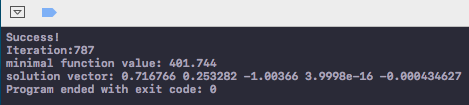
\includegraphics[scale = 0.7]{pic/3.png}
    \caption{ 算法运行结果, 函数最小值为401.744}
\end{figure}

可得函数最小值为401.744, 每个参数在最小值的取值分别为:

\begin{equation}
x_1=0.716766,\quad x_2=0.253282,\quad x_3=-1.00366,\quad x_4=3.9998\times10^{-16},\quad x_5=-0.000434627
\end{equation}

我们用 MATLAB 来进行验证, 将目标函数与线性约束输入进程序之后,得到最小化结果为:
\begin{figure}[htp]
    \centering
    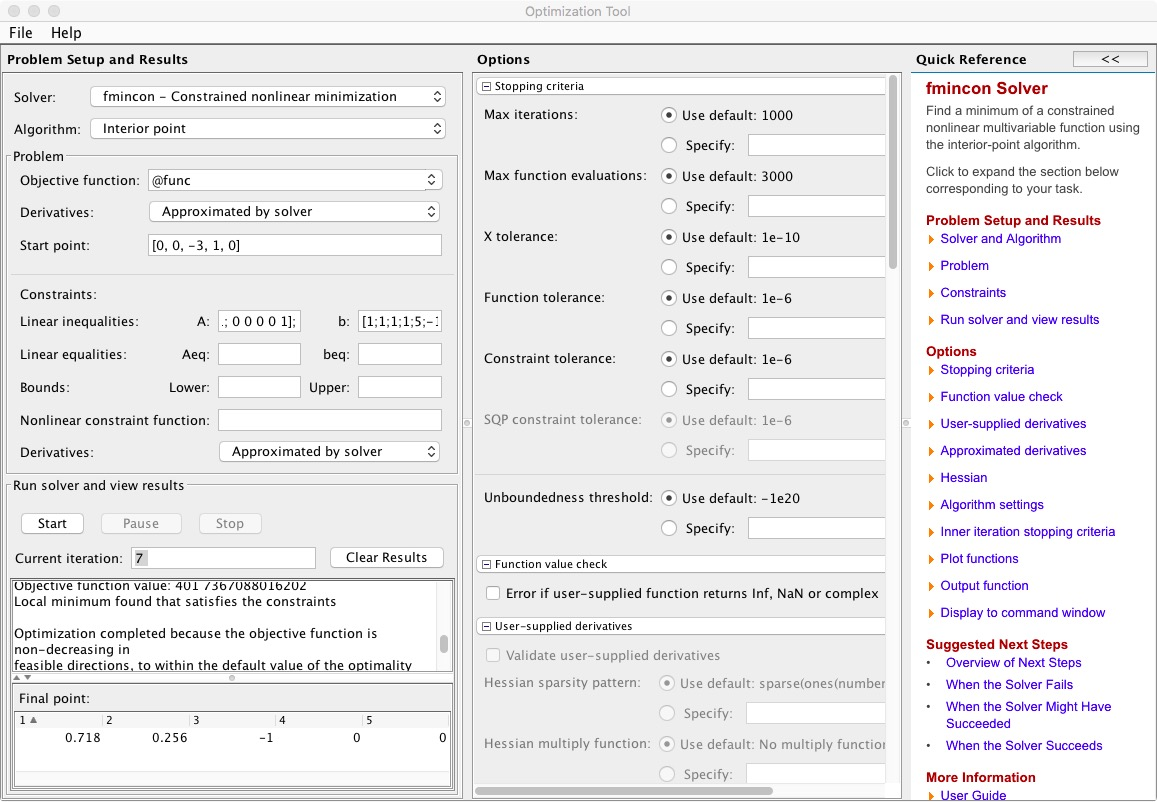
\includegraphics[scale = 0.3]{pic/4.jpeg}
    \caption{ MATLAB 运行结果}
\end{figure}

可见 MATLAB 对最小值的求解结果为401.7367088016202, 与我们给出的算法相差在0.01之内, 而它给出的参数对应值为:
\begin{equation}
x_1=0.718,\quad x_2=0.256,\quad x_3=-1,\quad x_4=0,\quad x_5=0
\end{equation}

只有$x_1,x_2$与标准相差在0.02$\sim$0.03之间,其余均在0.01的标准之下,可以认为我们已经得到了非常精确的最小值的解.
